
The limits for the cut based VBF channel are shown in 
Table~\ref{tab:uls_2j_cut} and Figure~\ref{fig:uls_2j_cut}.
The limits for the cut based analysis in all final states are shown in
Table~\ref{tab:ulscut} and Figure~\ref{fig:uls_cut}.
The BDT and 2D analyses in the 0 and 1-jet different flavor final states
are combined with the cut based VBF and same flavor analyses in
Tables~\ref{tab:uls_bdt01_cut2_cutsf} and~\ref{tab:uls_2d01_cut2_cutsf}
and Figures~\ref{fig:uls_bdt01_cut2_cutsf} and~\ref{fig:uls_2d01_cut2_cutsf} 
respectively.

%%%%%%%%%%%%%%%%%
% plot
\begin{figure}[!hbtp]
\centering
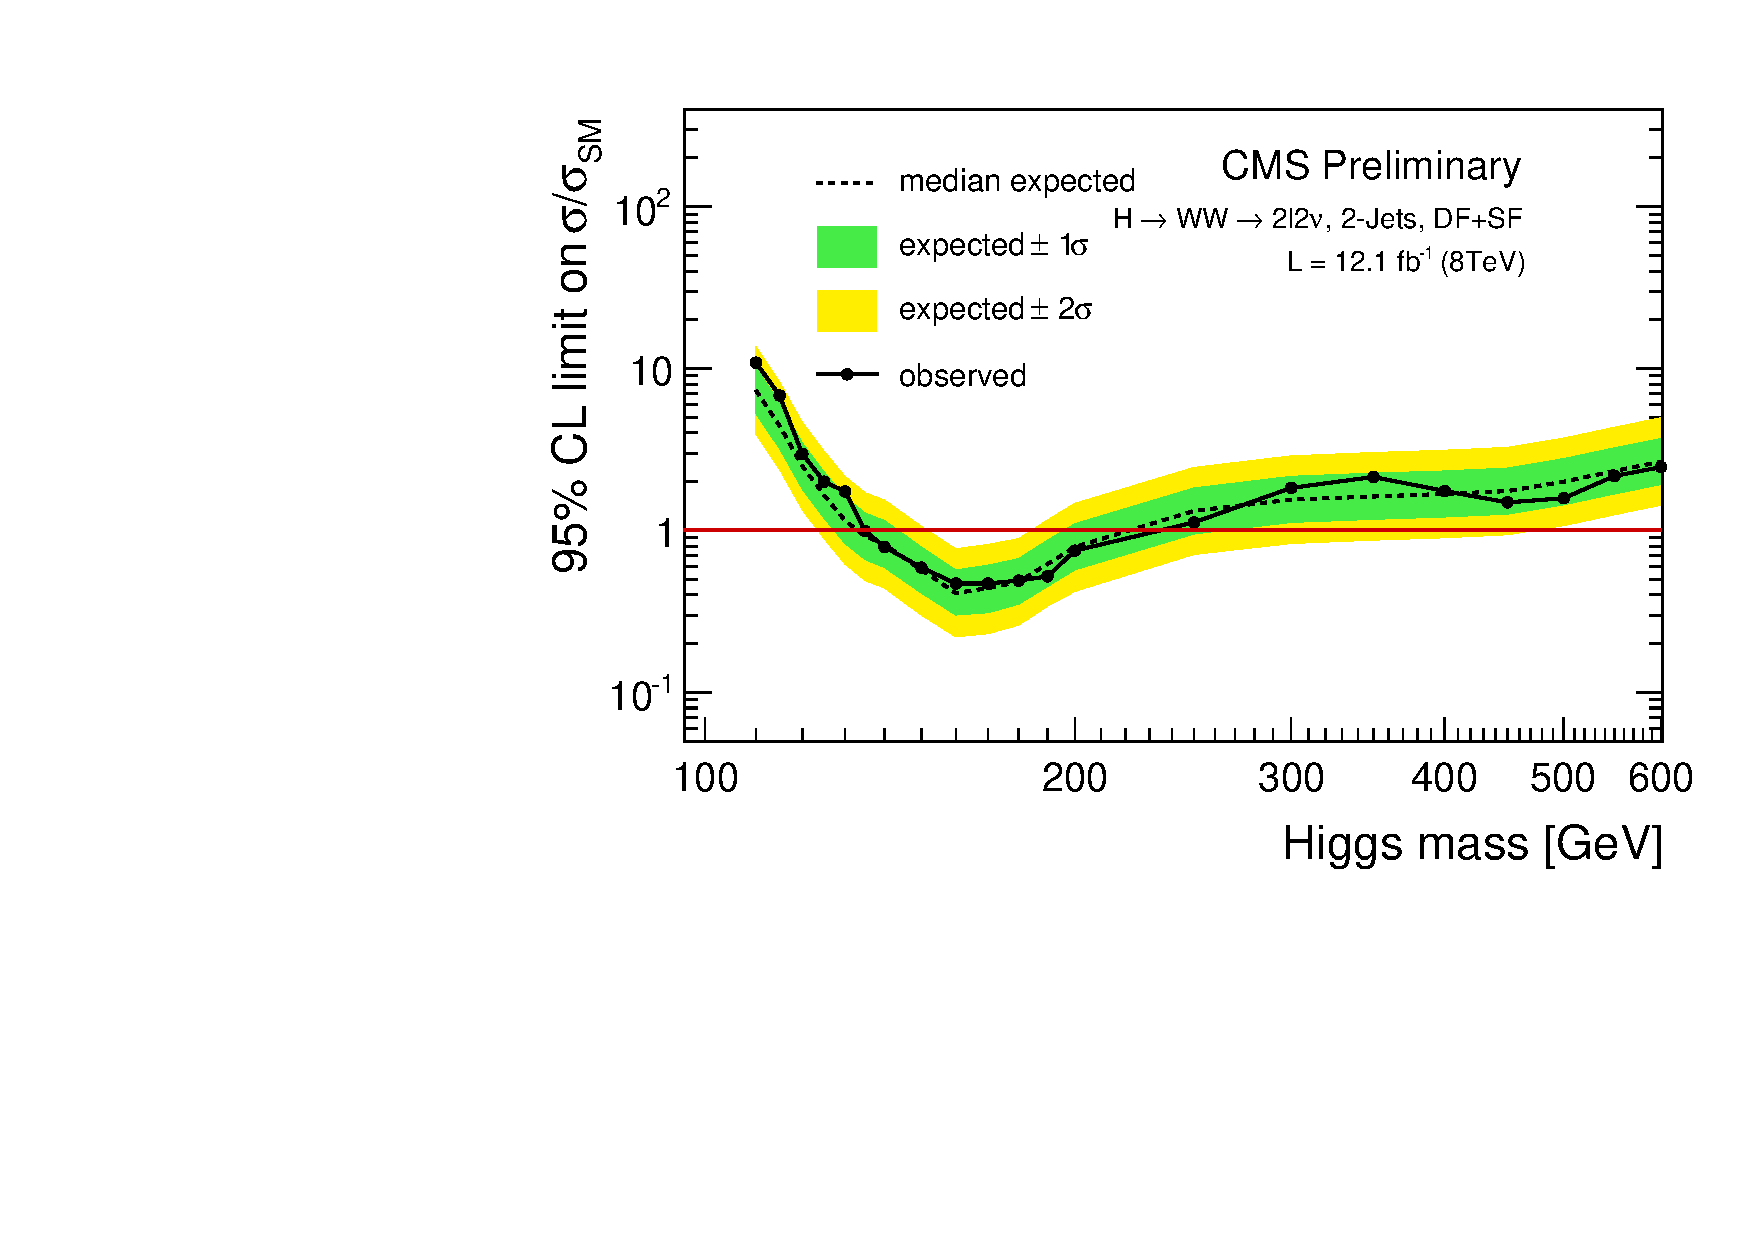
\includegraphics[width=.75\textwidth]{figures/table_limits_2j_cut_log.pdf}
\caption{Expected upper limits for SM Higgs in $\intlumiEightTeV$ at 8 TeV in the VBF channel.
The cut-based result is used. }
\label{fig:uls_2j_cut}
\end{figure}
% table
\begin{table}[!htbp]
\begin{center}
\begin{tabular}{c c c c c}
\hline
\vspace{-3mm} && \\
Higgs Mass & Observed  & Median expected & Expected range for 68\% & Expected range for 95\%   \\
\hline
110 & -1.00 & 7.95 & [5.73, 11.06] & [4.27, 14.83] \\
115 & -1.00 & 4.67 & [3.37, 6.50] & [2.51, 8.71] \\
120 & -1.00 & 2.60 & [1.88, 3.62] & [1.40, 4.86] \\
125 & -1.00 & 1.74 & [1.25, 2.42] & [0.93, 3.24] \\
130 & -1.00 & 1.19 & [0.85, 1.65] & [0.64, 2.21] \\
135 & -1.00 & 0.96 & [0.70, 1.34] & [0.52, 1.80] \\
140 & -1.00 & 0.82 & [0.59, 1.15] & [0.44, 1.54] \\
150 & -1.00 & 0.57 & [0.41, 0.80] & [0.31, 1.07] \\
160 & -1.00 & 0.41 & [0.30, 0.58] & [0.22, 0.77] \\
170 & -1.00 & 0.44 & [0.32, 0.61] & [0.24, 0.82] \\
180 & -1.00 & 0.49 & [0.35, 0.68] & [0.26, 0.91] \\
190 & -1.00 & 0.63 & [0.45, 0.88] & [0.34, 1.18] \\
200 & -1.00 & 0.81 & [0.58, 1.12] & [0.43, 1.50] \\
250 & -1.00 & 1.36 & [0.98, 1.89] & [0.73, 2.53] \\
300 & -1.00 & 1.57 & [1.13, 2.19] & [0.84, 2.93] \\
350 & -1.00 & 1.67 & [1.20, 2.33] & [0.90, 3.12] \\
400 & -1.00 & 1.78 & [1.28, 2.48] & [0.96, 3.32] \\
450 & -1.00 & 1.85 & [1.33, 2.57] & [0.99, 3.45] \\
500 & -1.00 & 2.15 & [1.55, 2.98] & [1.15, 4.00] \\
550 & -1.00 & 2.53 & [1.82, 3.52] & [1.36, 4.71] \\
600 & -1.00 & 2.95 & [2.13, 4.11] & [1.58, 5.50] \\
\vspace{-3mm} && \\
\hline
\end{tabular}
\caption{Expected upper limits for SM Higgs in $\intlumiEightTeV$ at 8 TeV in the VBF channel.
The cut-based result is used. }
\label{tab:uls_2j_cut}
\end{center}
\end{table}
%%%%%%%%%%

%%%%%%%%%%%%%%%%%
% plot
\begin{figure}[!hbtp]
\centering
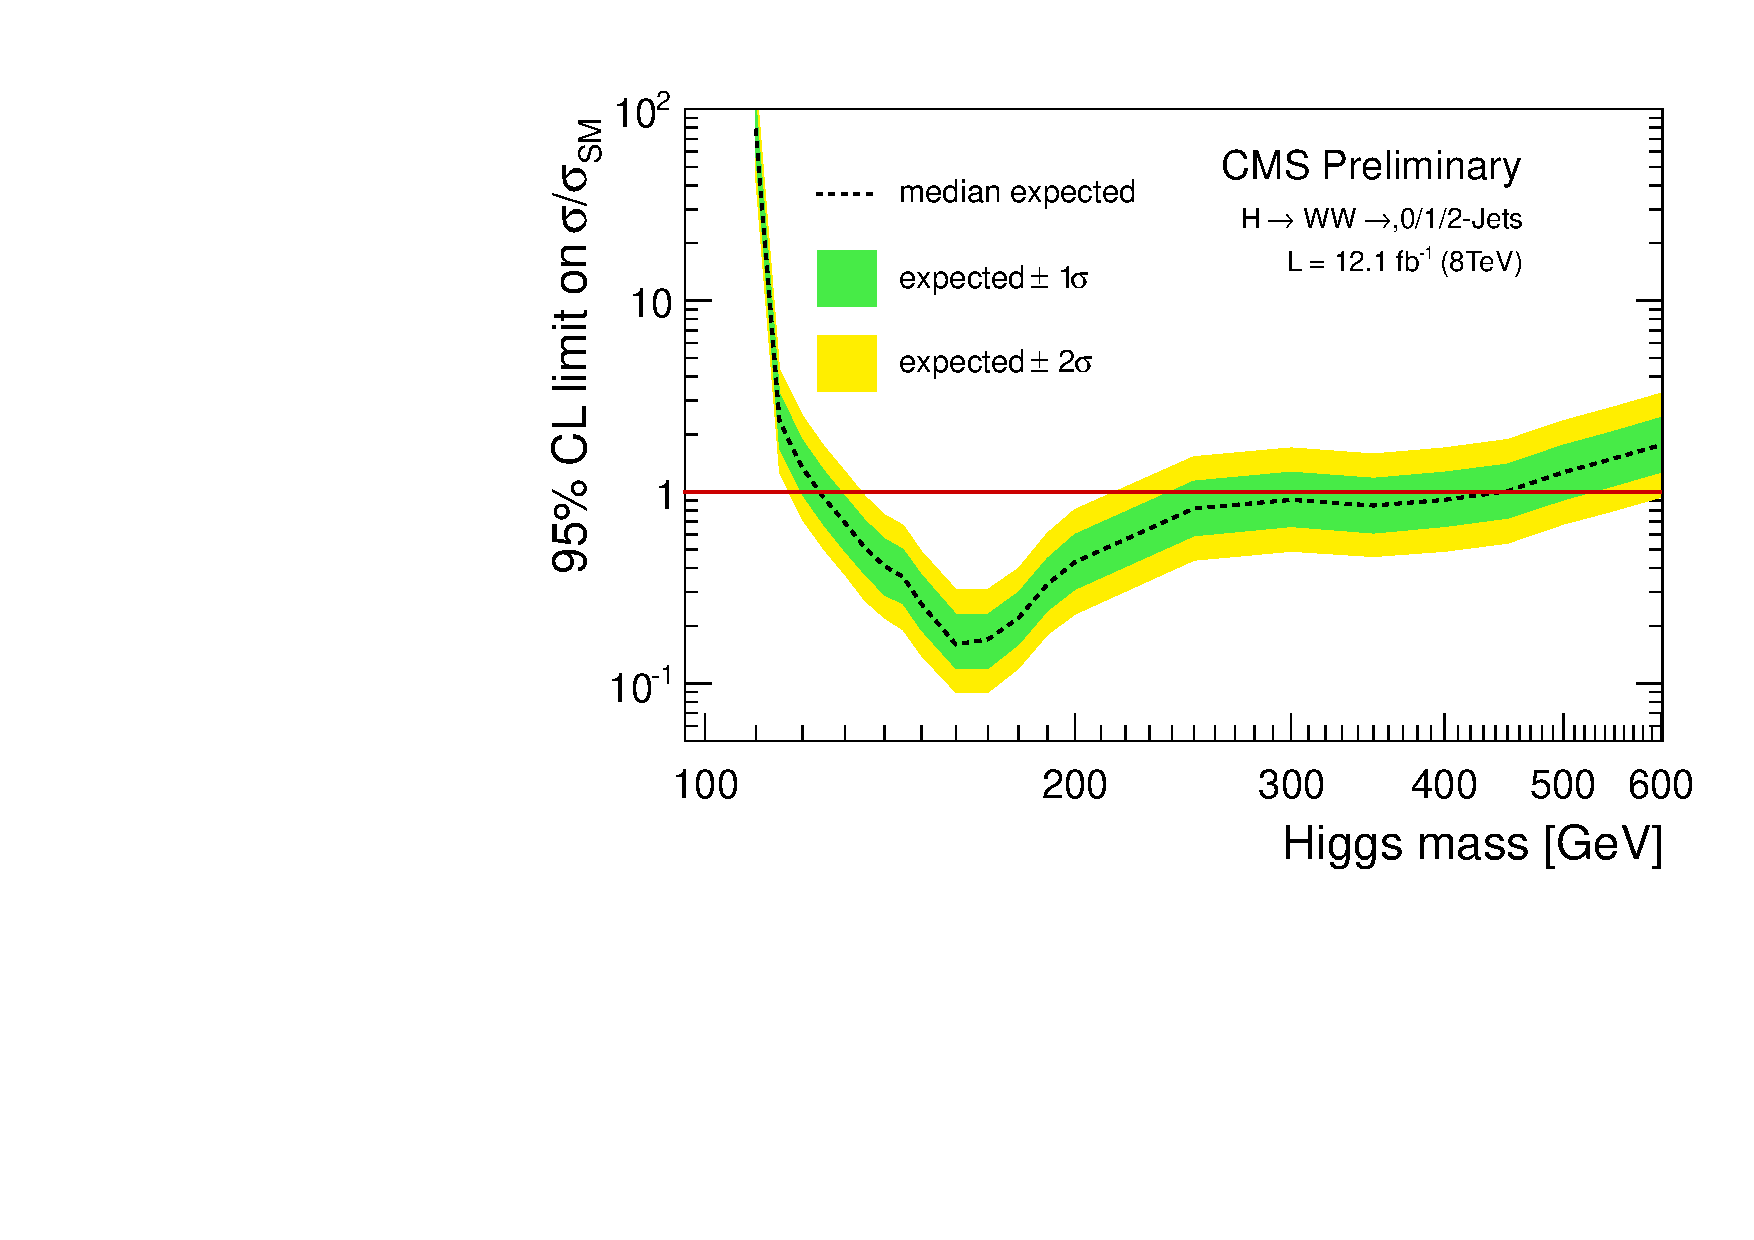
\includegraphics[width=.75\textwidth]{figures/table_limits_nj_cut_log.pdf}
\caption{Expected upper limits for SM Higgs in $\intlumiEightTeV$ at 8 TeV in all final states combined.
Cut-based result is used. }
\label{fig:uls_cut}
\end{figure}
% table
\begin{table}[!htbp]
\begin{center}
\begin{tabular}{c c c c c}
\hline
\vspace{-3mm} && \\
Higgs Mass & Observed  & Median expected & Expected range for 68\% & Expected range for 95\%   \\
\hline
110 & -1.00 & 4.61 & [3.32, 6.42] & [2.48, 8.61] \\
115 & -1.00 & 2.34 & [1.69, 3.26] & [1.26, 4.37] \\
120 & -1.00 & 1.34 & [0.97, 1.87] & [0.72, 2.51] \\
125 & -1.00 & 0.93 & [0.67, 1.29] & [0.50, 1.73] \\
130 & -1.00 & 0.69 & [0.49, 0.95] & [0.37, 1.28] \\
135 & -1.00 & 0.51 & [0.37, 0.71] & [0.27, 0.95] \\
140 & -1.00 & 0.41 & [0.29, 0.57] & [0.22, 0.76] \\
150 & -1.00 & 0.26 & [0.19, 0.37] & [0.14, 0.49] \\
160 & -1.00 & 0.16 & [0.12, 0.23] & [0.09, 0.31] \\
170 & -1.00 & 0.17 & [0.12, 0.23] & [0.09, 0.31] \\
180 & -1.00 & 0.22 & [0.16, 0.30] & [0.12, 0.40] \\
190 & -1.00 & 0.33 & [0.24, 0.45] & [0.18, 0.61] \\
200 & -1.00 & 0.43 & [0.31, 0.60] & [0.23, 0.81] \\
250 & -1.00 & 0.82 & [0.59, 1.14] & [0.44, 1.53] \\
300 & -1.00 & 0.91 & [0.66, 1.27] & [0.49, 1.70] \\
350 & -1.00 & 0.85 & [0.61, 1.18] & [0.46, 1.58] \\
400 & -1.00 & 0.91 & [0.66, 1.27] & [0.49, 1.70] \\
450 & -1.00 & 1.01 & [0.73, 1.40] & [0.54, 1.88] \\
500 & -1.00 & 1.27 & [0.91, 1.76] & [0.68, 2.36] \\
550 & -1.00 & 1.50 & [1.08, 2.08] & [0.80, 2.79] \\
600 & -1.00 & 1.76 & [1.27, 2.45] & [0.94, 3.28] \\
\vspace{-3mm} && \\
\hline
\end{tabular}
\caption{Expected upper limits for SM Higgs in $\intlumiEightTeV$ at 8 TeV in all final states combined.
Cut-based result is used. }
\label{tab:ulscut}
\end{center}
\end{table}
%%%%%%%%%%

%%%%%%%%%%%%%%%%%
% plot
\begin{figure}[!hbtp]
\centering
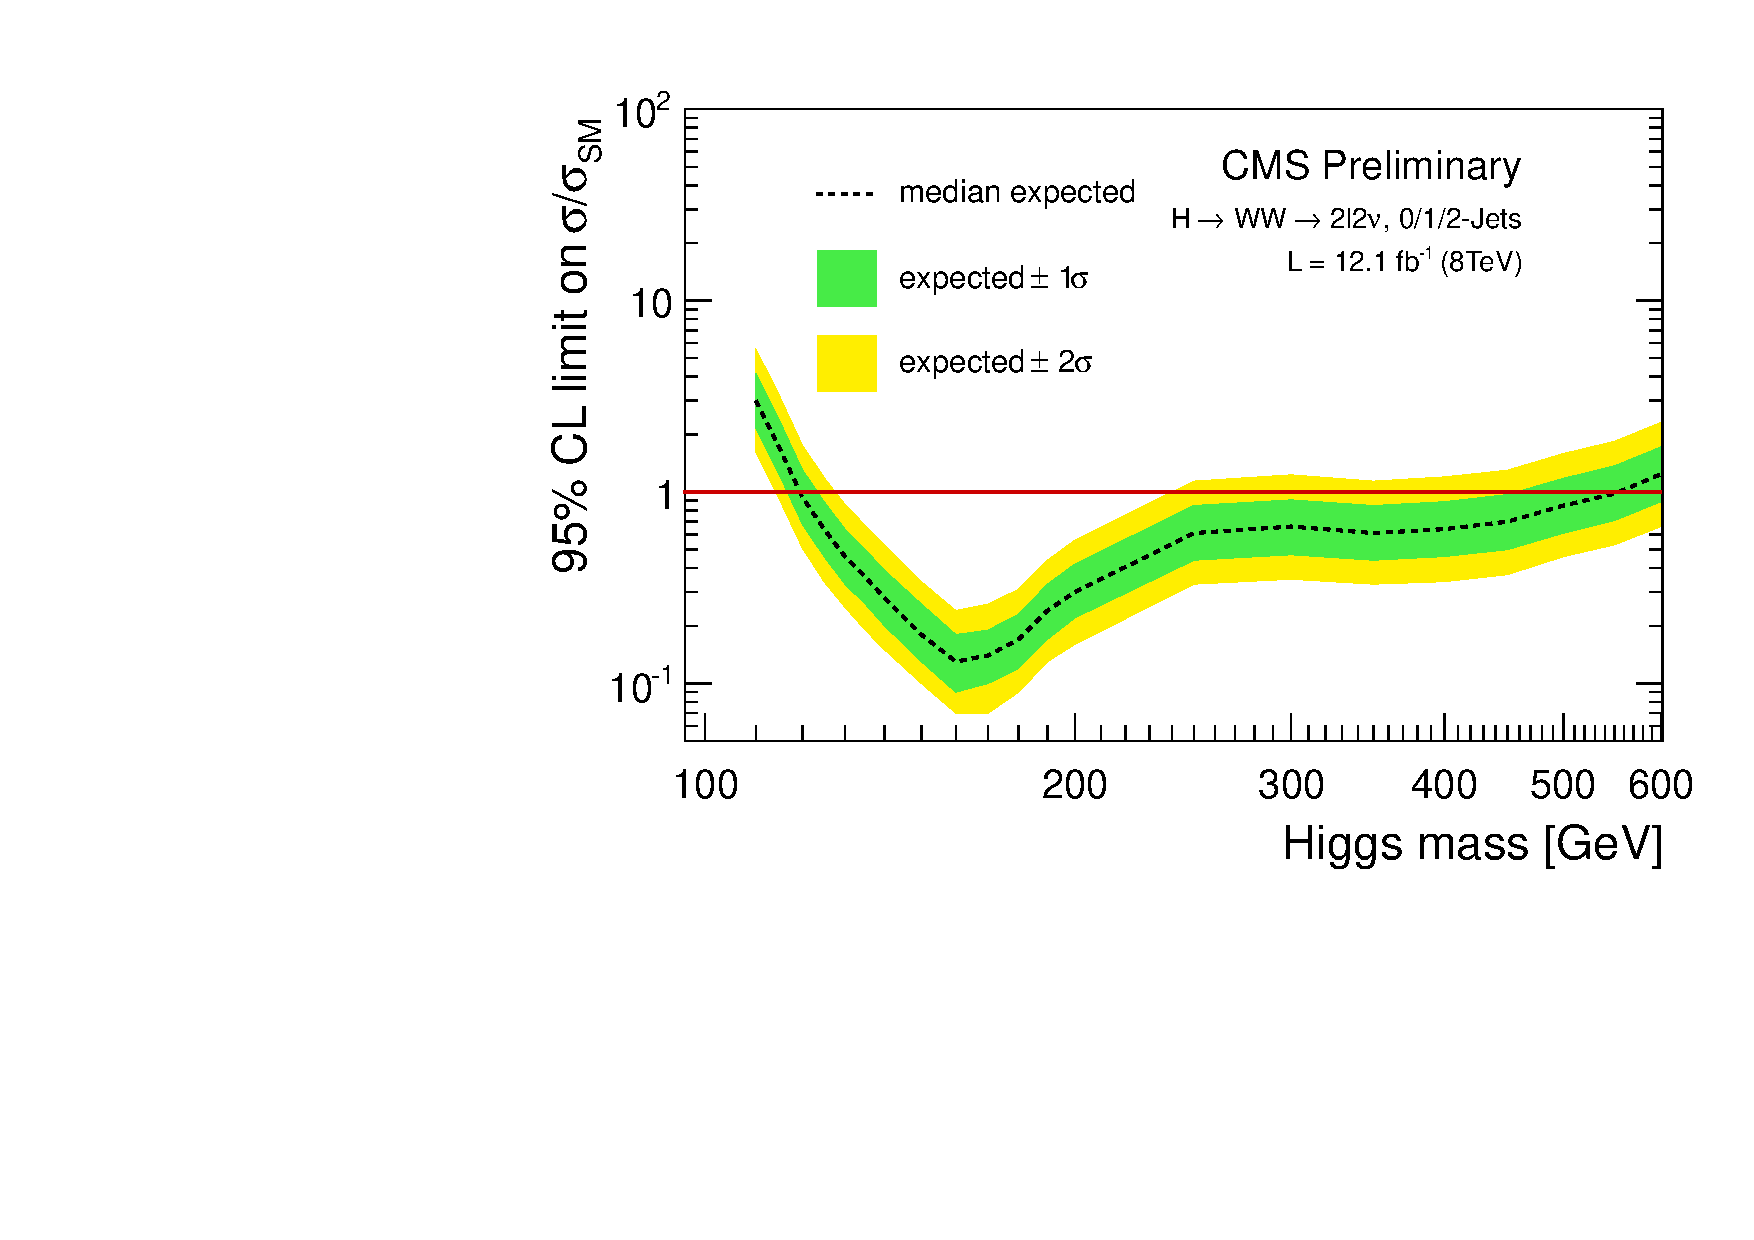
\includegraphics[width=.75\textwidth]{figures/table_limits_nj_shape_of_cut_log.pdf}
\caption{Expected upper limits for SM Higgs in $\intlumiEightTeV$ at 8 TeV.
BDT result is used for OF 0/1jet bin and cut-based result is used for VBF channel
and in the SF final states. }
\label{fig:uls_bdt01_cut2_cutsf}
\end{figure}
% table
\begin{table}[!htbp]
\begin{center}
\begin{tabular}{c c c c c}
\hline
\vspace{-3mm} && \\
Higgs Mass & Observed  & Median expected & Expected range for 68\% & Expected range for 95\%   \\
\hline
110 & -1.00 & 3.00 & [2.16, 4.18] & [1.61, 5.60] \\
115 & -1.00 & 1.70 & [1.22, 2.36] & [0.91, 3.17] \\
120 & -1.00 & 0.94 & [0.68, 1.31] & [0.51, 1.76] \\
125 & -1.00 & 0.64 & [0.46, 0.89] & [0.34, 1.19] \\
130 & -1.00 & 0.46 & [0.33, 0.64] & [0.25, 0.86] \\
135 & -1.00 & 0.36 & [0.26, 0.50] & [0.19, 0.67] \\
140 & -1.00 & 0.28 & [0.20, 0.39] & [0.15, 0.53] \\
150 & -1.00 & 0.18 & [0.13, 0.26] & [0.10, 0.34] \\
160 & -1.00 & 0.13 & [0.09, 0.18] & [0.07, 0.24] \\
170 & -1.00 & 0.14 & [0.10, 0.19] & [0.07, 0.26] \\
180 & -1.00 & 0.17 & [0.12, 0.23] & [0.09, 0.31] \\
190 & -1.00 & 0.24 & [0.17, 0.33] & [0.13, 0.44] \\
200 & -1.00 & 0.30 & [0.22, 0.42] & [0.16, 0.56] \\
250 & -1.00 & 0.61 & [0.44, 0.85] & [0.33, 1.14] \\
300 & -1.00 & 0.66 & [0.47, 0.91] & [0.35, 1.23] \\
350 & -1.00 & 0.61 & [0.44, 0.85] & [0.33, 1.14] \\
400 & -1.00 & 0.64 & [0.46, 0.89] & [0.34, 1.20] \\
450 & -1.00 & 0.70 & [0.50, 0.97] & [0.37, 1.30] \\
500 & -1.00 & 0.85 & [0.61, 1.18] & [0.46, 1.59] \\
550 & -1.00 & 0.98 & [0.71, 1.37] & [0.53, 1.84] \\
600 & -1.00 & 1.24 & [0.89, 1.72] & [0.66, 2.31] \\
\vspace{-3mm} && \\
\hline
\end{tabular}
\caption{Expected upper limits for SM Higgs in $\intlumiEightTeV$ at 8 TeV.
BDT result is used for OF 0/1jet bin and cut-based result is used for VBF channel
and in the SF final states. }
\label{tab:uls_bdt01_cut2_cutsf}
\end{center}
\end{table}
%%%%%%%%%%

%%%%%%%%%%%%%%%%%
% plot
\begin{figure}[!hbtp]
\centering
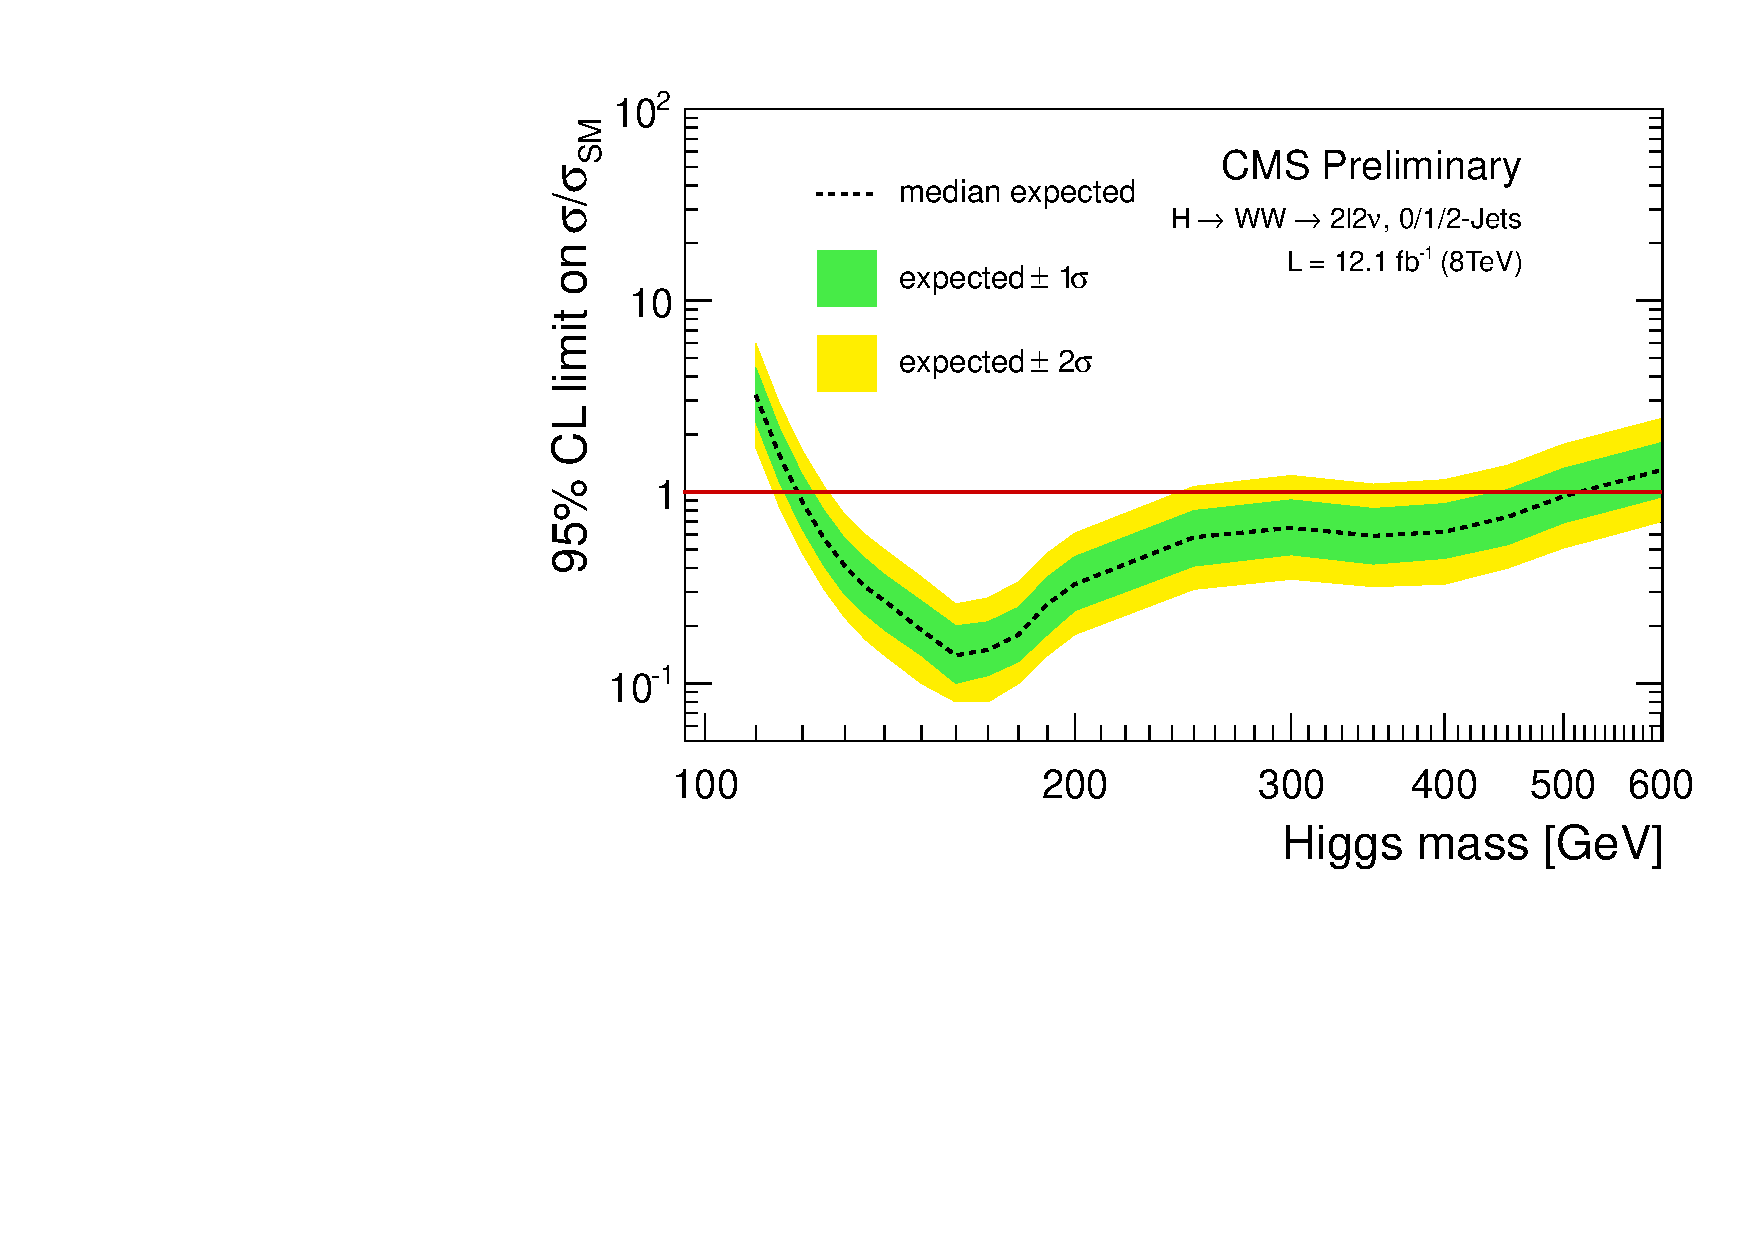
\includegraphics[width=.75\textwidth]{figures/table_limits_nj_shape2d_of_cut_log.pdf}
\caption{Expected upper limits for SM Higgs in $\intlumiEightTeV$ at 8 TeV.
2D result is used for OF 0/1jet bin and cut-based result is used for VBF channel
and in the SF final states. }
\label{fig:uls_2d01_cut2_cutsf}
\end{figure}
% table
\begin{table}[!htbp]
\begin{center}
\begin{tabular}{c c c c c}
\hline
\vspace{-3mm} && \\
Higgs Mass & Observed  & Median expected & Expected range for 68\% & Expected range for 95\%   \\
\hline
110 & -1.00 & 3.20 & [2.31, 4.46] & [1.70, 5.98] \\
115 & -1.00 & 1.55 & [1.12, 2.15] & [0.83, 2.89] \\
120 & -1.00 & 0.89 & [0.64, 1.23] & [0.48, 1.65] \\
125 & -1.00 & 0.57 & [0.41, 0.80] & [0.31, 1.07] \\
130 & -1.00 & 0.41 & [0.29, 0.57] & [0.22, 0.76] \\
135 & -1.00 & 0.32 & [0.23, 0.45] & [0.17, 0.60] \\
140 & -1.00 & 0.27 & [0.19, 0.37] & [0.14, 0.50] \\
150 & -1.00 & 0.19 & [0.14, 0.27] & [0.10, 0.36] \\
160 & -1.00 & 0.14 & [0.10, 0.20] & [0.08, 0.26] \\
170 & -1.00 & 0.15 & [0.11, 0.21] & [0.08, 0.28] \\
180 & -1.00 & 0.18 & [0.13, 0.25] & [0.10, 0.34] \\
190 & -1.00 & 0.26 & [0.18, 0.36] & [0.14, 0.48] \\
200 & -1.00 & 0.33 & [0.24, 0.46] & [0.18, 0.61] \\
250 & -1.00 & 0.58 & [0.41, 0.80] & [0.31, 1.07] \\
300 & -1.00 & 0.65 & [0.47, 0.91] & [0.35, 1.22] \\
350 & -1.00 & 0.59 & [0.42, 0.82] & [0.32, 1.10] \\
400 & -1.00 & 0.62 & [0.45, 0.87] & [0.33, 1.16] \\
450 & -1.00 & 0.74 & [0.53, 1.03] & [0.40, 1.38] \\
500 & -1.00 & 0.95 & [0.69, 1.33] & [0.51, 1.78] \\
550 & -1.00 & 1.12 & [0.81, 1.56] & [0.60, 2.09] \\
600 & -1.00 & 1.30 & [0.94, 1.81] & [0.70, 2.42] \\
\vspace{-3mm} && \\
\hline
\end{tabular}
\caption{Expected upper limits for SM Higgs in $\intlumiEightTeV$ at 8 TeV.
2D result is used for OF 0/1jet bin and cut-based result is used for VBF channel
and in the SF final states. }
\label{tab:uls_2d01_cut2_cutsf}
\end{center}
\end{table}
%%%%%%%%%%



